\documentclass{article}
% Note: Use the 'aastex631.cls' class file provided by AAS Journals.

\usepackage{amsmath,amssymb}
\usepackage{graphicx}
\usepackage{slashed}
\usepackage{tikz-feynman}
\usepackage{siunitx}
\usepackage{cite}

% Custom commands for convenience
\newcommand{\mN}{m_N}
\newcommand{\mmu}{m_\mu}
\newcommand{\mpi}{m_\pi}

\begin{document}

\title{Constraining Heavy Neutral Leptons with Multi-Messenger Observations of the Active Galactic Nucleus NGC 1068}

% % Author list formatted for ApJ
% \author{Liang Wei}
% \affiliation{School of Physics, East China Normal University, Shanghai 200241, China}

% \author{Jianhong Ruan}
% \affiliation{School of Physics, East China Normal University, Shanghai 200241, China}
% % You can add \email{...} for the corresponding author

% \begin{abstract}
% Recent observations by the IceCube Neutrino Observatory have identified the active galactic nucleus (AGN) NGC 1068 as a source of high-energy neutrinos. However, multimessenger data reveal that the corresponding $\gamma$-ray flux is significantly attenuated, highlighting the difficulty conventional electromagnetic cascade models face in explaining the opacity of the AGN corona. In this paper, we investigate the Heavy Neutral Lepton (HNL) scenario as a potential mechanism to bypass this obscured region. Introduced via the Inverse Seesaw (ISS) mechanism, HNLs can be produced in the high-energy AGN environment. We calculate the detailed kinematics, branching ratios, and helicity distributions of HNLs produced from pion and muon decays. We subsequently evaluate the energy spectra of decay products from HNLs in both leptonic and radiative decay channels. Applying this framework to NGC 1068, we estimate the HNL transport and their subsequent conversion into observable $\gamma$-rays. Our results indicate that if HNLs decay purely via the ISS-driven leptonic channel (producing secondary electrons that undergo inverse Compton scattering), the resulting $\gamma$-ray flux is orders of magnitude below current detection thresholds. Conversely, if HNLs possess a dominant dipole radiative decay channel, they can partially account for the observed high-energy $\gamma$-ray excess. Based on this, we derive upper-limit constraints on the HNL-$\nu_\mu$ mixing angle $|U_\mu|^2$, demonstrating the potential of AGN multimessenger observations to probe physics beyond the Standard Model.
% \end{abstract}

% \keywords{Active galactic nuclei (16) --- Neutrino astronomy (1100) --- High-energy astrophysics (739) --- Beyond the Standard Model (1545)}

\section{Introduction} \label{sec:intro}

The continuous advancement of observational techniques has ushered in a rich era of multimessenger astronomy. Among the various cosmic messengers, high-energy neutrinos play a critical role, as they provide a direct window into the extreme non-thermal processes occurring in distant astrophysical sources. Neutrinos themselves act as an anomaly within the Standard Model (SM), and investigating their mass generation mechanisms and interactions serves as a pivotal gateway to Beyond the Standard Model (BSM) physics.

A landmark discovery in this context is the recent confirmation by the IceCube collaboration of the active galactic nucleus (AGN) NGC 1068 as a high-energy neutrino point source \cite{icecube2022evidence}. Similar observatories, such as KM3NeT/ARCA, are currently expanding our observational capabilities in the TeV--PeV range, particularly for the Southern Hemisphere \cite{km3net2024astronomy, km3net2025observation}.

When comparing the IceCube neutrino observations of NGC 1068 with theoretical predictions \cite[e.g.,][]{murase2020hidden}, a striking tension emerges: the high-energy $\gamma$-ray flux is significantly suppressed relative to the neutrino flux. This implies that the AGN core (the corona region) is highly opaque to high-energy $\gamma$-rays. Conventional electromagnetic cascade models can only partially explain this $\gamma$-ray attenuation. An intriguing alternative is the presence of weakly interacting particles that can escape the opaque core and subsequently decay into observable photons. Axion-like particles (ALPs) have been discussed in this context \cite{pant2024constraining}. Similarly, Heavy Neutral Leptons (HNLs)—often introduced in Type-I or Inverse Seesaw (ISS) models to explain neutrino masses \cite{king2025righthandedneutrinosseesawmodels}—present a compelling candidate. 

Due to their long lifetimes, HNLs are notoriously difficult to detect in laboratory experiments, though significant constraints exist \cite{bryman2019constraints}. However, large-scale astrophysical environments offer a distinct advantage. Previous studies have used supernova SN 1987A to constrain HNL parameter space \cite{Magill_2018}. In this work, we apply this concept to the AGN NGC 1068.

We systematically calculate the production of HNLs via pion and muon decays in the AGN core, paying special attention to the helicity distributions and mass-induced kinematics. We then calculate the resulting energy spectra from both leptonic and radiative decay channels. Finally, we apply these theoretical derivations to the observational data of NGC 1068 to evaluate the phenomenological viability of HNLs and to establish constraints on the mixing angle $|U_\mu|^2$.

\section{Theoretical Framework of HNLs} \label{sec:theory}

Before exploring observable signatures in astrophysical environments, we establish the theoretical framework governing HNL production and decay. 

\subsection{HNL Origin: The Inverse Seesaw Mechanism} \label{sec:iss}

In a simplified Type-I Seesaw model, adding a right-handed neutrino field allows for a Dirac mass $m_D$ and a Majorana mass $M_R$. Diagonalization yields the active neutrino mass $m_\nu \simeq m_D^2/M_R$, HNL mass $m_N \simeq M_R$, and mixing angle $|U|^2 \simeq (m_D/M_R)^2$. The strong coupling between HNL mass and mixing angle makes detection extremely challenging for most of the parameter space.

This limitation is bypassed by the Inverse Seesaw (ISS) mechanism, which introduces an additional fermion field $S$ with a small Majorana mass term $\mu$ that breaks lepton number conservation. The mass matrix becomes:
\begin{equation}
  \begin{pmatrix}
    0   & m_D & 0    \\
    m_D & 0   & M    \\
    0   & M   & \mu
  \end{pmatrix}
\end{equation}
Assuming $M \gg m_D \gg \mu$, the neutrino mass, HNL mass, and mixing angle are given by \cite{king2025righthandedneutrinosseesawmodels}:
\begin{equation}
  m_\nu = \mu \frac{m_D^2}{M^2}, \quad m_N \simeq M, \quad |U|^2 = \frac{m_\nu}{\mu}.
\end{equation}
By decoupling the mixing angle from the HNL mass through the parameter $\mu$, the ISS mechanism can naturally explain sub-eV neutrino masses while allowing for phenomenologically accessible HNL masses and mixing angles.

\subsection{HNL Production Kinematics} \label{sec:production}

In the high-energy AGN environment, abundant pions are generated via $pp$ and $p\gamma$ interactions. Through mixing $U_{\mu}$, these pions (and their subsequent muons) can decay into HNLs.

\subsubsection{Pion Decay ($\pi^\pm \to \mu^\pm N$)}

The decay width for HNL production relative to SM neutrino production is modified by the mixing angle and a kinematic factor:
\begin{equation}
  \frac{\Gamma_{\pi \to \mu N}}{\Gamma_{\pi \to \mu \nu}} = |U_{\mu}|^2 \times \rho_\pi (m_N), \label{eq:pion_HNL_rho}
\end{equation}
where
\begin{equation}
   \rho_\pi (m_N) = \frac{(\mpi^2 (\mmu^2 + \mN^2) - (\mmu^2 - \mN^2)^2) \sqrt{\lambda(\mpi^2, \mmu^2, \mN^2)}}{\mmu^2 (\mpi^2 - \mmu^2)^2}, \label{eq:rho_pi}
\end{equation}
and $\lambda(x, y, z) = x^2 + y^2 + z^2 - 2xy - 2yz - 2zx$. For $m_N \in [10, 30]$ MeV, $\rho_\pi(m_N)$ decreases from approximately 1 to 0.7.

The maximum fraction of energy an HNL can carry in the laboratory frame is:
\begin{equation}
  \lambda_{max} = \frac{E_{N,max}}{E_\pi} = \frac{\mpi^2 - \mmu^2 + \mN^2 + \sqrt{\lambda(\mpi^2, \mmu^2, \mN^2)}}{2 \mpi^2}.
\end{equation}
For $m_N \in [10, 30]$ MeV, this ratio drops from 0.42 to 0.34, meaning massive HNLs carry slightly less energy from pions compared to massless neutrinos ($\sim 0.43$). Following \cite{kelner2006energy}, the HNL spectrum for a known pion spectrum $J(E_\pi)$ is:
\begin{equation}
  Q_{N}(E_N) = \int_{\frac{E_N}{\lambda_{max}}}^{\infty} J(E_\pi) \frac{d E_\pi}{\lambda_{max} E_\pi}. \label{eq:hnl_spec_from_pion}
\end{equation}

In the pion rest frame, the ratio of right-handed ($\Gamma_R$) to left-handed ($\Gamma_L$) HNL production is given by:
\begin{equation}
  \frac{\Gamma_R}{\Gamma_L} = \frac{(\mmu^2 + \mN^2) \mpi^2 - (\mmu^2 - \mN^2)^2 - (\mmu^2 - \mN^2) \sqrt{\lambda}}
  {(\mmu^2 + \mN^2) \mpi^2 - (\mmu^2 - \mN^2)^2 + (\mmu^2 - \mN^2) \sqrt{\lambda}}. \label{eq:hnl_hel_pion}
\end{equation}

\subsubsection{Muon Decay ($\mu^- \to e^- \bar{\nu}_e N$)}

For the three-body muon decay, the relative width is:
\begin{equation}
  \frac{\Gamma_{\mu \to N}}{\Gamma_{\mu \to \nu}} = |U_{\mu}|^2 \times \rho_\mu(m_N),
\end{equation}
where the kinematic suppression factor (with $r_N = m_N / m_\mu$) is \cite{Bondarenko_2018}:
\begin{equation}
  \rho_\mu(m_N) = - r_N^8 + 8 r_N^6 - 24 r_N^4 \ln(r_N) - 8 r_N^2 + 1. \label{eq:rho_mu}
\end{equation}
The HNL energy spectrum in the muon rest frame is:
\begin{equation}
  \frac{d\Gamma}{dE} = \frac{G_F^2 p^2 (3 \mmu^2 E + 3 \mN^2 E - 4 \mmu p - 6 \mN^2 \mmu)}{12 \pi^3 E}. \label{eq:mu_HNL_spec}
\end{equation}
Averaging over muon polarization, the decay width into an HNL with helicity $s$ is:
\begin{equation}
  \begin{split}
    \Gamma_{\mu \to N}^{(s)} \propto \; & s \cdot (r_N^8-32 r_N^5+90 r_N^4-96 r_N^3+40 r_N^2-3) \\ 
                                        & -72 r_N^4 \, \ln{(r_N)} -3 r_N^8+24 r_N^6-24 r_N^2+3.
  \end{split} \label{eq:mu_HNL_pol}
\end{equation}
Depending on $m_N$, the majority of HNLs produced are left-handed.

\subsection{HNL Lifetime and Decay Channels} \label{sec:decay}

\subsubsection{Leptonic Decay}
In the considered mass range, HNLs decay via the neutral current ($Z^0$) mixing with $\nu_\mu$. The relevant channels are $N \to 3\nu$ and $N \to \nu_\mu e^- e^+$. Ignoring the electron mass, the widths are \cite{Bondarenko_2018}:
\begin{align}
  \Gamma_{N \to 3\nu}          & = \frac{G_F^2 m_N^5}{192 \pi^3} |U_\mu|^2, \label{eq:HNL_3nu_decay} \\
  \Gamma_{N \to \nu e \bar{e}} & = \frac{G_F^2 m_N^5}{192 \pi^3} |U_\mu|^2 C_1^e, \label{eq:HNL_nuee_decay}
\end{align}
where $C_1^e = \frac{1}{4}(1 - 4 \sin^2 \theta_W + 8 \sin^4 \theta_W)$. The branching ratio to electrons is $BR \approx 0.11$. Due to this small branching ratio and the suppression of the weak interaction, the leptonic decay channel significantly limits the efficiency of energy transfer to observable photons. 

\subsubsection{Radiative Decay}
While flavor-changing neutral currents are GIM-suppressed in standard ISS models, introducing an effective non-renormalizable dipole operator provides a direct radiative decay channel \cite{Magill_2018}:
\begin{equation}
  \mathcal{L}_{int} = \frac{d}{2} \bar{\nu}_L \sigma_{\mu \nu} F^{\mu \nu} N + h.c. \label{eq:int_mag_nu}
\end{equation}
This interaction yields a width $\Gamma_{N \to \nu \gamma} = \frac{|d|^2 m_N^3}{8 \pi}$. In the HNL rest frame, considering initial polarization, the angular distribution of the emitted photon is $d \Gamma / d \Omega \propto 1 + \cos{\theta_{s}}$.

If we assume all HNLs are purely left-handed (an approximation valid at low masses, though Eq.~\ref{eq:hnl_hel_pion} gives precise values), the laboratory frame $\gamma$-ray spectrum in the relativistic limit simplifies to:
\begin{equation}
  Q_\gamma^{(Lab)} (E) = \int_{E}^{+\infty}d E_N \, Q_N(E_N) \, \frac{2 (E_N - E)}{E_N^2}. \label{eq:pure_L_N_gamma}
\end{equation}

\section{Application to NGC 1068} \label{sec:application}

\subsection{Multimessenger Context}
NGC 1068 is located at approximately 14.4 Mpc. In standard astrophysical models, $pp$ and $p\gamma$ interactions in the AGN environment generate comparable fluxes of high-energy neutrinos and $\gamma$-rays. However, observations reveal a "neutrino-bright, $\gamma$-ray-dim" scenario \cite{murase2020hidden}. The HNL scenario posits that HNLs, produced abundantly alongside neutrinos, escape the opaque corona due to their weak interactions and long lifetimes. Once outside, their decays can generate observable $\gamma$-ray signatures.

\subsection{Flux Estimation and Constraints}

Based on \cite{icecube2022evidence}, the muon neutrino flux from NGC 1068 is modeled as a power law:
\begin{equation}
  \Phi_{\nu_\mu + \bar{\nu}_\mu} = \Phi_0 \left(\frac{E_\nu}{E_0}\right)^{-\gamma}. \label{eq:icecube_nuspec}
\end{equation}
As a first-order phenomenological approximation for $m_N \leq 30$ MeV, we scale the SM neutrino flux to estimate the HNL flux, assuming similar kinematics:
\begin{equation}
  \Phi_N (E) \approx |U_\mu|^2 (\rho_\pi + \rho_\mu) \Phi_{\nu_\mu + \bar{\nu}_\mu} (E). \label{eq:approx_spec}
\end{equation}

If HNLs decay purely via the leptonic channel (Eq.~\ref{eq:HNL_nuee_decay}), the resulting high-energy electrons must undergo inverse Compton (IC) scattering with the cosmic microwave background to produce $\gamma$-rays. Under a simple $\delta$-function approximation for IC scattering ($E_\gamma \approx \frac{4}{3} (E_e/m_e)^2 \epsilon_0$), the cascade process significantly degrades the energy. Our estimations show that this flux is several orders of magnitude below current detection thresholds, rendering the purely ISS leptonic decay model untestable with current NGC 1068 data.

Conversely, if the dipole radiative decay (Eq.~\ref{eq:int_mag_nu}) dominates, the energy is directly transferred to $\gamma$-rays. Applying Eq.~\ref{eq:pure_L_N_gamma}, the resulting $\gamma$-ray spectrum undergoes kinematic broadening. By ensuring this predicted flux does not exceed the observed $\gamma$-ray upper limits for NGC 1068 \cite{murase2020hidden}, we can place constraints on the parameter space. Assuming dipole dominance, we derive an upper limit on the mixing angle $|U_\mu|^2 \lesssim 10^{-2}$ for specific mass regimes (see Figures \ref{fig:gamma_spec_U_2} and \ref{fig:U_UL_approx}). 

\begin{figure}[htbp]
  \centering
  % Replace with your actual graphic files
  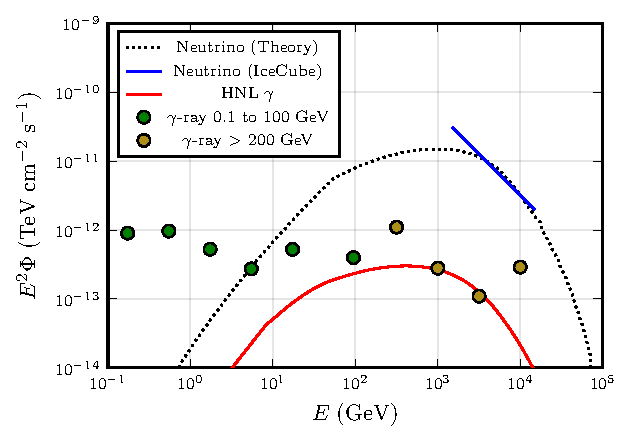
\includegraphics[width=0.45\textwidth]{julia_plots/u1.5_gamma.pdf} 
  \caption{Estimated $\gamma$-ray fluxes from HNL decays in NGC 1068, under the assumption of a dominant dipole radiative decay channel. The model is compared with IceCube data and cascade predictions.}
  \label{fig:gamma_spec_U_2}
\end{figure}

\begin{figure}[htbp]
  \centering
  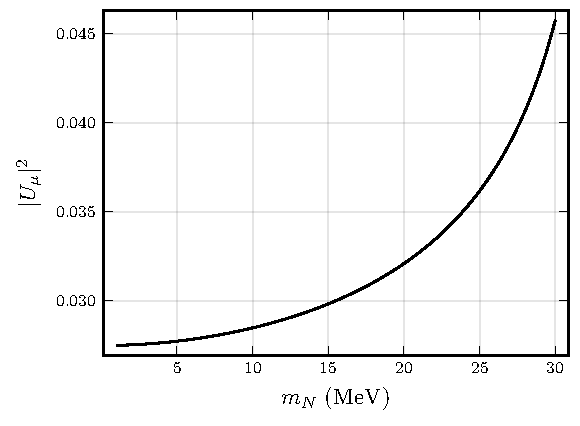
\includegraphics[width=0.45\textwidth]{julia_plots/U_UL.pdf}
  \caption{Derived upper limits on the HNL mixing angle $|U_\mu|^2$ based on NGC 1068 $\gamma$-ray constraints, assuming dominant radiative decay.}
  \label{fig:U_UL_approx}
\end{figure}

\section{Conclusions} \label{sec:conclusion}

In this paper, we explored the Heavy Neutral Lepton (HNL) scenario to address the multimessenger anomaly observed in the AGN NGC 1068, where the high-energy $\gamma$-ray flux is significantly suppressed relative to the neutrino flux. 

We conducted detailed phenomenological calculations of HNL production kinematics, helicity distributions, and decay spectra for $m_N \leq 30$ MeV. Our application of this framework to NGC 1068 yields two main conclusions:
1. If HNLs decay strictly through SM-mixed leptonic channels, the resulting secondary IC $\gamma$-ray flux is heavily suppressed and remains far below observational thresholds.
2. If BSM dipole operators enable a dominant radiative decay channel, HNLs can efficiently transport energy out of the opaque corona and partially explain the observable $\gamma$-ray signals. Under this assumption, we constrained the mixing angle to $|U_\mu|^2 \lesssim 10^{-2}$.

Future observations from next-generation observatories like KM3NeT/ARCA and the Cherenkov Telescope Array (CTA), combined with full 3D Monte Carlo transport simulations integrating our derived helicity specific equations, will further compress this parameter space and potentially reveal definitive BSM signatures in extreme astrophysical environments.


\appendix

\section{Derivation of HNL Production and Decay Amplitudes} \label{sec:appendix}

In this appendix, we outline the calculation of the squared matrix elements incorporating HNL spin polarization.

\subsection{Pion Decay ($\pi \to \mu N$)}
The amplitude for pion decay is given by:
\begin{equation}
  \mathcal{M} = \frac{f_\pi g_w^2}{8 M_W^2} k^\mu [\bar{u}(p_2) \gamma_\mu (1 - \gamma^5) v(p_1)].
\end{equation}
To retain the final-state HNL spin information, we utilize the projection operator:
\begin{equation}
  u(p_2) \bar{u}(p_2) = (\slashed{p}_2 + m_N) \frac{1 + \slashed{s}}{2},
\end{equation}
where $s^\mu$ is the HNL spin four-vector. In the pion rest frame, boosting from the HNL rest frame yields $s^\mu = \left(\frac{|p_2|}{m_N} s, 0, 0, \frac{\sqrt{|p_2|^2 + m_N^2}}{m_N} s\right)$, with $s = \pm 1$. The squared amplitude is:
\begin{equation}
  \langle |\mathcal{M}| \rangle^2 = \frac{1}{16} \left[ f_\pi^2 \left( \frac{g_w}{M_W} \right)^2 \right]^2 [ 2 (k \cdot p_1) (k \cdot p_2) - k^2 (p_1 \cdot p_2) + 2 m_N (k \cdot p_1) (k \cdot s) - m_N k^2 (p_1 \cdot s) ].
\end{equation}
Evaluating this kinematically yields the helicity-dependent widths in Eq.~\ref{eq:hnl_hel_pion}.

\subsection{Muon Decay ($\mu \to e \nu e N$)}
The amplitude is:
\begin{equation}
  \mathcal{M} = 2\sqrt{2} G_F [\bar{u}(p_1) \gamma_\mu P_L u(k)] \cdot [\bar{u}(p_2) \gamma^\mu P_L v(p_3) ].
\end{equation}
Retaining the HNL spin, the trace calculation simplifies to:
\begin{equation}
  \langle |\mathcal{M}| \rangle^2 = 32 G_F [(k \cdot p_3)(p_1 \cdot p_2) - m_N (k \cdot p_3) (p_2 \cdot s)].
\end{equation}
Eliminating $p_2$ and integrating over the three-body phase space using a $\delta$-function yields the mass suppression factor $\rho_\mu(m_N)$ (Eq.~\ref{eq:rho_mu}) and the polarized width (Eq.~\ref{eq:mu_HNL_pol}).

\subsection{Radiative Decay ($N \to \nu \gamma$)}
For the dipole interaction operator, the Feynman vertex is $i \, 2 \, d \, \sigma^{\alpha\beta} q_\beta P_R$. The decay amplitude is:
\begin{equation}
  \mathcal{M} = 2i \, d [\bar{u}(p_1) \sigma^{\alpha\beta} p_{2\beta} P_R u(k)] \epsilon_\alpha(p_2).
\end{equation}
Taking the squared modulus:
\begin{equation}
  \langle |\mathcal{M}| \rangle^2 = 4 |d|^2 m_N^3 [m_N + 2 (p_2 \cdot s)].
\end{equation}
Substituting $p_2 \cdot s = \frac{m_N}{2} \cos{\theta_s}$ yields the angular distribution $\propto 1 + \cos{\theta_s}$.

\bibliographystyle{ieeetr}
\bibliography{ref}
\end{document}